\chapter{Los pulmones y el intercambio de gases}\label{ch:g7:lungs-and-gas-exchange}

Cada minuto de tu vida, unos ocho litros de aire pasan por dos órganos
que no has visto nunca. El \cref{ch:g4:breathing} esbozó el camino y el
intercambio; el \cref{ch:g7:how-animals-breathe} colocó la máquina
humana entre las cuatro del reino. Este capítulo completa el cuadro: la
maquinaria de \omterm{def:g7:what-is-respiration:respiration}{ventilación}, las bolsas de aire con su nombre propio, los
números del intercambio --- y lo que le hace el humo a todo el conjunto.

\section{La maquinaria de ventilación}

\begin{proposition}[Cómo se mueve el aire]\label{prop:g7:lungs-and-gas-exchange:ventilation}
Los \omterm{def:g7:how-animals-breathe:four}{pulmones} no tienen \omterm{def:g3:bones-and-muscles:muscle}{músculos} propios; el pecho los bombea como un
fuelle:
\begin{itemize}
  \item tomar aire es \emph{trabajo}: los \omterm{def:g3:bones-and-muscles:muscle}{músculos} de las \omterm{def:g3:bones-and-muscles:skeleton}{costillas}
        levantan y ensanchan la caja, y el
        \emph{diafragma}\index{diafragma} --- el ancho piso muscular
        que hay debajo de los \omterm{def:g7:how-animals-breathe:four}{pulmones} --- se aplana hacia abajo; el
        pecho ensanchado estira los \omterm{def:g7:how-animals-breathe:four}{pulmones} y el aire entra a
        llenarlos;
  \item soltar aire, en reposo, es sobre todo \emph{soltar}: los
        \omterm{def:g3:bones-and-muscles:muscle}{músculos} se relajan, el pecho estirado recupera su forma y el
        aire sale. (Apagar velas de un soplido le añade \omterm{def:g3:bones-and-muscles:muscle}{músculo} al
        muelle.)
\end{itemize}
Unas $15$ veces por minuto en reposo
(\cref{def:g4:breathing:movements}), sin que se lo pidan
(\cref{rem:g5:brain-in-command:more}) --- y más profundo y más rápido
cuando hace falta (\cref{prop:g7:organs-at-work:supply}).
\end{proposition}
\admitted

\begin{example}[Notar el fuelle]\label{ex:g7:lungs-and-gas-exchange:feel}
Con las manos en las \omterm{def:g3:bones-and-muscles:skeleton}{costillas}, toma aire hondo: la caja sube y se
ensancha bajo tus palmas (\cref{ex:g4:breathing:watch}). Ahora jadea
como un perro: esos soplidos rápidos y superficiales son casi todos
\omterm{prop:g7:lungs-and-gas-exchange:ventilation}{diafragma}. Y el hipo, para completar, son los falsos arranques
espasmódicos del \omterm{prop:g7:lungs-and-gas-exchange:ventilation}{diafragma} --- el fuelle fallando a su propio ritmo.
\end{example}

\section{Los alvéolos y el intercambio}

\begin{definition}[Alvéolos]\label{def:g7:lungs-and-gas-exchange:alveoli}
Las bolsitas de aire de la \cref{def:g4:breathing:organs} son los
\emph{alvéolos}\index{alvéolo}: cientos de millones de burbujas de
pared fina agrupadas en las puntas más finas de las vías respiratorias,
cada una envuelta en \omterm{def:g4:heart-and-blood:vessels}{vasos sanguíneos} finos. Su superficie sumada es la
media pista de tenis de la \cref{rem:g4:breathing:sponge} --- la copia
humana del pliego de \omterm{def:g6:exploring-our-environment:conditions}{condiciones} de grande, fina y húmeda de la
\cref{prop:g7:how-animals-breathe:spec}.
\end{definition}

\begin{proposition}[El intercambio, en números]\label{prop:g7:lungs-and-gas-exchange:numbers}
Compara el aire que entra con el aire que sale: el aire inspirado tiene
alrededor del $21$ por ciento de \omterm{def:g7:what-is-respiration:respiration}{oxígeno} y casi nada de \omterm{def:g7:what-is-respiration:respiration}{dióxido de
carbono}; el aire espirado baja hasta alrededor del $16$ por ciento de
\omterm{def:g7:what-is-respiration:respiration}{oxígeno} y sube hasta alrededor del $4$ por ciento de \omterm{def:g7:what-is-respiration:respiration}{dióxido de carbono}
(además de cálido y húmedo --- \cref{ex:g4:breathing:mirror}). Las
diferencias son el intercambio: a través de las paredes alveolares, el
\omterm{def:g7:what-is-respiration:respiration}{oxígeno} pasa a la \omterm{prop:g4:journey-of-food:absorb}{sangre} y el \omterm{def:g7:what-is-respiration:respiration}{dióxido de carbono} pasa de vuelta
(\cref{prop:g4:breathing:exchange}), cada minuto de cada día.
\end{proposition}
\admitted

\begin{omfigure}
\begin{tikzpicture}
  \node[anchor=south west, inner sep=0] (img) at (0,0)
    {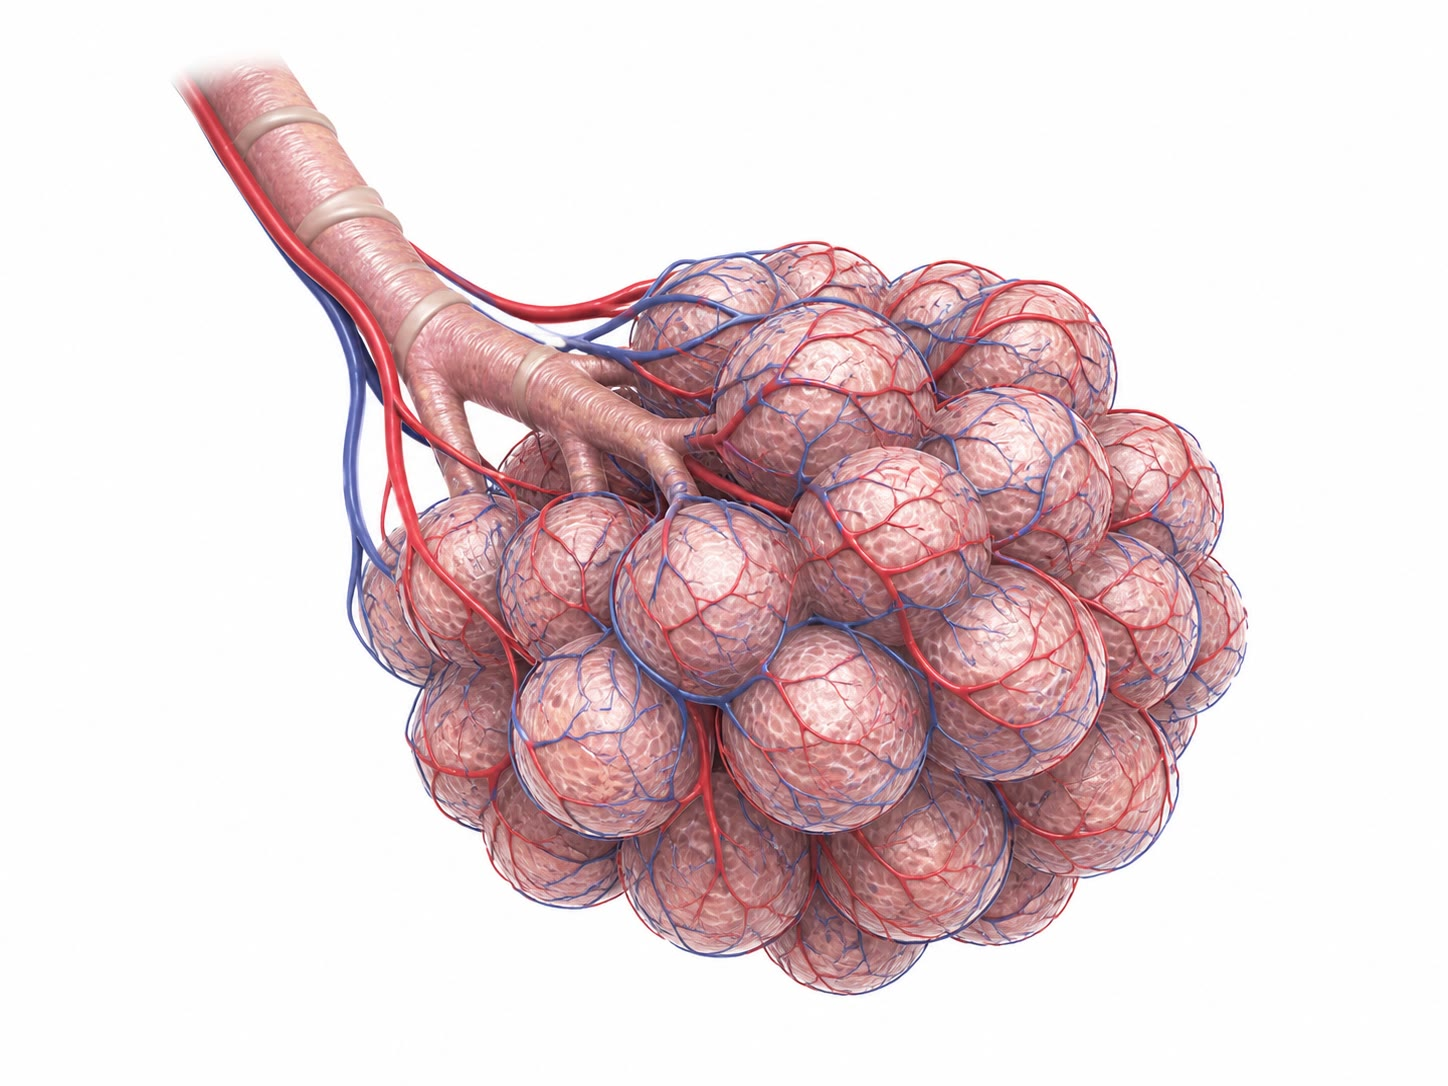
\includegraphics[width=0.6\linewidth]{images/book1/ai/fig-alveoli.jpg}};
  \begin{scope}[x={(img.south east)}, y={(img.north west)},
      every node/.style={font=\small}]
    \draw[omDef, thick] (0.24,0.83) -- (0.12,0.94)
      node[above] {vía respiratoria más fina};
    \draw[omThm, thick] (0.78,0.62) -- (0.90,0.80)
      node[above, align=center, omThm] {los vasos finos\\ que la envuelven};
    \draw[omMeth!60!black, thick] (0.46,0.34) -- (0.30,0.01)
      node[below, align=center, omMeth!60!black]
      {por la pared fina de cada burbuja:\\ el oxígeno a la sangre y el dióxido\\
       de carbono de vuelta al aire};
  \end{scope}
\end{tikzpicture}

{\small Un racimo de \omterm{def:g7:lungs-and-gas-exchange:alveoli}{alvéolos} de los cientos de millones: paredes finas
de burbuja, una envoltura de \omterm{def:g4:heart-and-blood:vessels}{vasos} finos y el paso en los dos sentidos
que es el sentido de todo esto.}
\end{omfigure}

\begin{example}[Las cuentas cuadran]\label{ex:g7:lungs-and-gas-exchange:accounting}
Ocho litros por minuto, con una veinteava parte del \omterm{def:g7:what-is-respiration:respiration}{oxígeno} de cada
\omterm{def:g7:what-is-respiration:respiration}{respiración} retenida: la aritmética cubre más o menos la factura de
\omterm{def:g7:what-is-respiration:respiration}{oxígeno} del cuerpo en reposo --- y en el esfuerzo, con la \omterm{def:g7:what-is-respiration:respiration}{ventilación}
triplicada y más profunda y las rondas del \omterm{def:g4:heart-and-blood:heart}{corazón} aceleradas
(\cref{prop:g7:organs-at-work:supply}), el reparto se multiplica hasta
igualar la factura de los \omterm{def:g3:bones-and-muscles:muscle}{músculos}. Los números de la máquina y la
contabilidad del cuerpo cuadran; son los mismos libros llevados en dos
mostradores.
\end{example}

\section{La maquinaria maltratada: el humo}

\begin{proposition}[Lo que le hace el humo al conjunto]\label{prop:g7:lungs-and-gas-exchange:smoke}
El humo del tabaco ataca todos los pisos de este capítulo (la
\cref{prop:g5:healthy-choices:substances} dio el aviso; aquí está la
ingeniería):
\begin{itemize}
  \item sus alquitranes recubren e irritan las vías respiratorias: las
        superficies de limpieza flaquean y la ``tos del fumador'' es la
        escoba sobrecargada de las vías;
  \item las paredes alveolares, irritadas de forma crónica, se
        deshacen: las bolsas se funden en espacios menos numerosos, más
        grandes y más flácidos --- \emph{se pierde superficie} y, con
        ella, intercambio (el pliego de \omterm{def:g6:exploring-our-environment:conditions}{condiciones}, desmontado);
  \item uno de los gases del humo ocupa los asientos del \omterm{def:g7:what-is-respiration:respiration}{oxígeno} en la
        \omterm{prop:g4:journey-of-food:absorb}{sangre} y desplaza al \omterm{def:g7:what-is-respiration:respiration}{oxígeno} de su propio transporte;
  \item y las vías respiratorias se estrechan --- cada \omterm{def:g7:what-is-respiration:respiration}{respiración} por
        el pecho de un fumador es una \omterm{def:g7:what-is-respiration:respiration}{respiración} por un fuelle medio
        atascado.
\end{itemize}
El daño es lento, acumulativo y solo reversible en parte: el \omterm{def:g7:how-animals-breathe:four}{pulmón} que
no empezó nunca conserva entera su media pista de tenis
(\cref{rem:g5:healthy-choices:never}).
\end{proposition}
\admitted

\begin{example}[Dos pruebas de escaleras]\label{ex:g7:lungs-and-gas-exchange:stairs}
Los tres pisos del \cref{ch:g7:organs-at-work}, subidos por dos adultos
de la misma edad y con las mismas costumbres de entrenamiento, uno de
ellos fumador desde hace mucho: el fumador llega jadeando con un \omterm{prop:g4:heart-and-blood:pulse}{pulso}
al que el otro solo llega esprintando. Menos superficie, asientos
ocupados, vías estrechadas --- la cadena de suministro paga la factura
de la \cref{prop:g7:organs-at-work:bill} por una toma estrangulada. Las
pruebas de forma física leen la historia de unos \omterm{def:g7:how-animals-breathe:four}{pulmones} con tanta
seguridad como cualquier escáner.
\end{example}

\begin{method}[Conservar la maquinaria]\label{met:g7:lungs-and-gas-exchange:keep}
El \cref{met:g4:breathing:care}, mejorado con las razones de este
capítulo:
\begin{enumerate}
  \item nada de humo --- ni tuyo ni de los demás: la superficie perdida
        casi no se recupera;
  \item ventila las habitaciones (\cref{exo:g4:breathing:10}) y elige
        aire limpio de la calle para el deporte;
  \item ejercita el fuelle: el esfuerzo que obliga a respirar hondo
        construye los \omterm{def:g3:bones-and-muscles:muscle}{músculos} respiratorios y mantiene ventilada toda
        la superficie;
  \item respira por la nariz con frío y con polvo
        (\cref{exo:g4:breathing:7}) --- el filtro protege a la escoba.
\end{enumerate}
\end{method}

\section{Ejercicios}

\begin{exercise}[$\star$]\label{exo:g7:lungs-and-gas-exchange:1}
Describe tomar aire y soltar aire como trabajo y como soltar: ¿qué
\omterm{def:g3:bones-and-muscles:muscle}{músculos} y qué movimientos?
\end{exercise}

\begin{exercise}[$\star$]\label{exo:g7:lungs-and-gas-exchange:2}
¿Qué es el \omterm{prop:g7:lungs-and-gas-exchange:ventilation}{diafragma} y dónde está?
\end{exercise}

\begin{exercise}[$\star$]\label{exo:g7:lungs-and-gas-exchange:3}
¿Qué son los \omterm{def:g7:lungs-and-gas-exchange:alveoli}{alvéolos} --- cuántos, con qué paredes y envueltos en qué?
\end{exercise}

\begin{exercise}[$\star$]\label{exo:g7:lungs-and-gas-exchange:4}
Da los números redondos: \omterm{def:g7:what-is-respiration:respiration}{oxígeno} del aire inspirado y del aire
espirado; \omterm{def:g7:what-is-respiration:respiration}{dióxido de carbono} del aire espirado. ¿Cuáles son las
diferencias?
\end{exercise}

\begin{exercise}[$\star$]\label{exo:g7:lungs-and-gas-exchange:5}
¿Qué pliego de \omterm{def:g6:exploring-our-environment:conditions}{condiciones} cumplen los \omterm{def:g7:lungs-and-gas-exchange:alveoli}{alvéolos} y con qué otros dos
órganos de este curso lo comparten?
\end{exercise}

\begin{exercise}[$\star$]\label{exo:g7:lungs-and-gas-exchange:6}
Nombra tres de los cuatro ataques del humo a la maquinaria.
\end{exercise}

\begin{exercise}[$\star\star$]\label{exo:g7:lungs-and-gas-exchange:7}
¿Por qué es trabajo tomar aire mientras que soltarlo en reposo sale
gratis? ¿De dónde viene el empujón hacia fuera?
\end{exercise}

\begin{exercise}[$\star\star$]\label{exo:g7:lungs-and-gas-exchange:8}
Explica por qué la superficie alveolar perdida no se puede compensar
respirando más deprisa --- ¿qué factor del intercambio falta?
\end{exercise}

\begin{exercise}[$\star\star$]\label{exo:g7:lungs-and-gas-exchange:9}
Interpreta las dos pruebas de escaleras del
\cref{ex:g7:lungs-and-gas-exchange:stairs} ataque por ataque.
\end{exercise}

\begin{exercise}[$\star\star$]\label{exo:g7:lungs-and-gas-exchange:10}
Un buceador suelta el aire despacio mientras sube; un trompetista
sostiene notas largas y constantes. ¿Qué mitades de la
\cref{prop:g7:lungs-and-gas-exchange:ventilation} está entrenando o
usando cada uno?
\end{exercise}

\begin{exercise}[$\star\star$]\label{exo:g7:lungs-and-gas-exchange:11}
Reconcilia el \cref{ex:g7:lungs-and-gas-exchange:accounting} con la
\cref{prop:g7:organs-at-work:supply}: ¿qué tres ajustes multiplican el
reparto en el esfuerzo y en qué mostradores?
\end{exercise}

\begin{exercise}[$\star\star\star$]\label{exo:g7:lungs-and-gas-exchange:12}
``El \omterm{def:g7:how-animals-breathe:four}{pulmón} es una frontera de media pista de tenis plegada dentro de
una caja de zapatos, y el humo es un fuego lento en la frontera''.
Justifica las dos imágenes con los números y los mecanismos de este
capítulo.
\end{exercise}

\section{Problema: El expediente de la máquina de respirar}

\begin{problem}[{Problema de fin de semana --- la inspección de una
ingeniera al fuelle humano}]\label{pb:g7:lungs-and-gas-exchange:1}
Una clase de ingeniería ``inspecciona'' sobre el papel la máquina
humana de respirar: toma, bomba, superficie de intercambio, conexión de
transporte y \omterm{def:g1:plants-around-us:parts}{hoja} de mantenimiento.

\medskip\noindent\textbf{Parte I --- La bomba.}
\begin{enumerate}
  \item Monta el ciclo de la bomba: las dos fases, los que mueven cada
        una y qué fase cuesta \omterm{prop:g3:balanced-diet:jobs}{energía} en reposo.
  \item La bomba no toca el \omterm{def:g3:bones-and-muscles:muscle}{músculo} del propio órgano bombeado --- los
        \omterm{def:g7:how-animals-breathe:four}{pulmones} no tienen ninguno. ¿Cómo mueve aire entonces el
        ensanchamiento del pecho?
  \item Da el ritmo en reposo de la bomba y sus dos ajustes de esfuerzo
        (\cref{prop:g7:organs-at-work:supply}).
  \item Jadear, suspirar, apagar velas de un soplido: asigna cada cosa
        a su sitio en la mecánica del ciclo.
\end{enumerate}

\medskip\noindent\textbf{Parte II --- La superficie de intercambio.}
\begin{enumerate}[resume]
  \item Especifica la superficie: nombre, número, pared, envoltura y
        tamaño sumado.
  \item Comprueba el pliego de \omterm{def:g6:exploring-our-environment:conditions}{condiciones} frente a la
        \cref{prop:g7:how-animals-breathe:spec}, punto por punto.
  \item El aire de entrada y el de salida se diferencian en los
        porcentajes del capítulo. Calcula la diferencia de \omterm{def:g7:what-is-respiration:respiration}{oxígeno} como
        fracción del $21$ por ciento de la entrada --- ¿qué parte del
        \omterm{def:g7:what-is-respiration:respiration}{oxígeno} inspirado se retiene, más o menos?
  \item ¿Por qué tiene que salir el aire de escape cálido y húmedo ---
        de qué propiedad de la superficie es ese el precio?
\end{enumerate}

\medskip\noindent\textbf{Parte III --- La \omterm{def:g1:plants-around-us:parts}{hoja} de mantenimiento.}
\begin{enumerate}[resume]
  \item Archiva los cuatro ataques del humo bajo: toma, bomba,
        superficie y transporte. Una línea para cada uno.
  \item El expediente anota: ``las pérdidas de superficie son pérdidas
        de capital''. Explícalo, frente a las toses y los resfriados,
        que son reparaciones corrientes.
  \item Escribe el plan de mantenimiento --- el
        \cref{met:g7:lungs-and-gas-exchange:keep} --- como cuatro
        directrices de ingeniería con sus razones.
  \item Cierra la inspección: una frase sobre por qué esta máquina, la
        única entre las bombas y las fronteras del cuerpo, está medio
        bajo el control voluntario de su dueño --- y para qué sirve ese
        control (el habla, el canto, la exhalación lenta del buceador).
\end{enumerate}
\end{problem}
